\chapter{Description du projet PongIO}
\label{chap:premier chapitre}

\section{État de l'art}
Le jeu Pong est un des premiers jeux d'arcade mais le tout premier en rapport avec le sport. Le jeu fut développé et commercialisé par Atari en Novembre 1972. Les règles du jeu sont très simples : chaque joueur s'affronte en déplaçant la raquette de haut en bas, via un bouton rotatif, de façon à renvoyer la balle dans le but adverse. Le joueur peut changer la direction de la balle en fonction de l'endroit où celle-ci tape sur la raquette, alors que sa vitesse augmente graduellement au cours de la manche. Un score est affiché pour la partie en cours et des bruitages accompagnent la frappe de la balle sur les raquettes. C'est donc un jeu inspiré du tennis de table en vue du dessus dont voici une illustration:

\begin{figure}[H]
  \center
  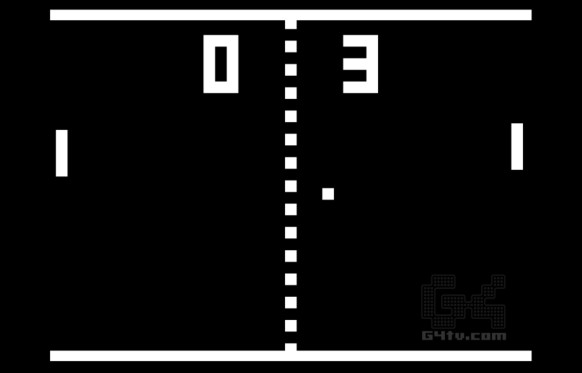
\includegraphics[width=5cm]{images/pong}
  \centering
  \caption{Illustration du jeu Pong. On voit à droite les rectangles correspondant aux raquettes des joueurs. La balle correspond au carré blanc proche du centre de l'image. Le score est affiché en haut de l'écran.}
  \label{fig:une-image}
\end{figure}


Le jeu à d'ailleurs rapporté plus de 40 millions de dollars de chiffres d'affaires en 1975. Ce succès est considéré comme l'évènement précurseur de l'industrie du jeu vidéo. Notre choix s'est porté sur ce jeu pour cette même raison. C'est également dans le but de tester nos compétences en programmation que nous nous sommes fixés comme but de donner à ce jeu "classique" une touche moderne et innovatrice, c'est pourquoi nous avons décidé d'en faire un jeu ".io".\\
Les jeux ".io" ont vu le jour grâce au jeu d'action massivement multijoueur AgarIO dont le succès fut tout simplement fulgurant. En effet durant sa première année de sortie il fut l'un des jeux les plus populaires que soit pour son site ou pour son application mobile. Dans ce jeu le joueur contrôle une cellule dans une carte où il doit manger un maximum de cellules pour devenir le plus gros possible. Puis de nombreux autres jeux ont suivi la tendance comme SlitherIO, VertixIO et plusieurs autres. Il y a de nombreuses raisons au succès de ses différents jeux ".io". Tout d'abord l'accessibilité de ces jeux les rend jouables n'importe où dans le monde. Le domaine ".io" dorénavant culte est très simple a mémoriser pour la majorité des gens. De plus, son prix n'est pas très élevé pour les développeurs comparé à d'autres domaines, ce qui rend les publicités suffisamment rentable. En effet, la gratuité implique que plus de joueurs peuvent y jouer. Finalement, le plus important, le fait que le jeu soit multijoueur permet aux joueurs du monde entier de s'affronter.\\


\section{Principe du PongIO}


La principale motivation qui nous a poussé à créer PongIO est le désir de moderniser et de redéfinir le mythique jeu qu'est Pong. Ainsi, en conservant les mécaniques de base, nous avons élargi les possibilités de varier les modes de jeu. PongIO ne se limite pas seulement à un affrontement de deux joueurs, nous avons implémenté différents modes de jeu allant du 2 contre 2 à chacun pour soi mais en allant jusqu'à 10 joueurs : ils sont ainsi placé sur un plateau hexagonal.


Nous avons décidé d'accorder une grande importance au graphisme de notre jeu pour qu'il puisse se distinguer suffisamment du Pong classique et qu'il apporte au joueur une expérience de jeu nouvelle et inédite. Nous avons choisi de nous orienter vers un design du jeu pixelisé. Le résultat s'accordait de façon impressionnante à notre idée du design pour la page de lancement du jeu. Voici une illustration de notre écran de lancement de partie:

\begin{figure}[H]
  \centering
  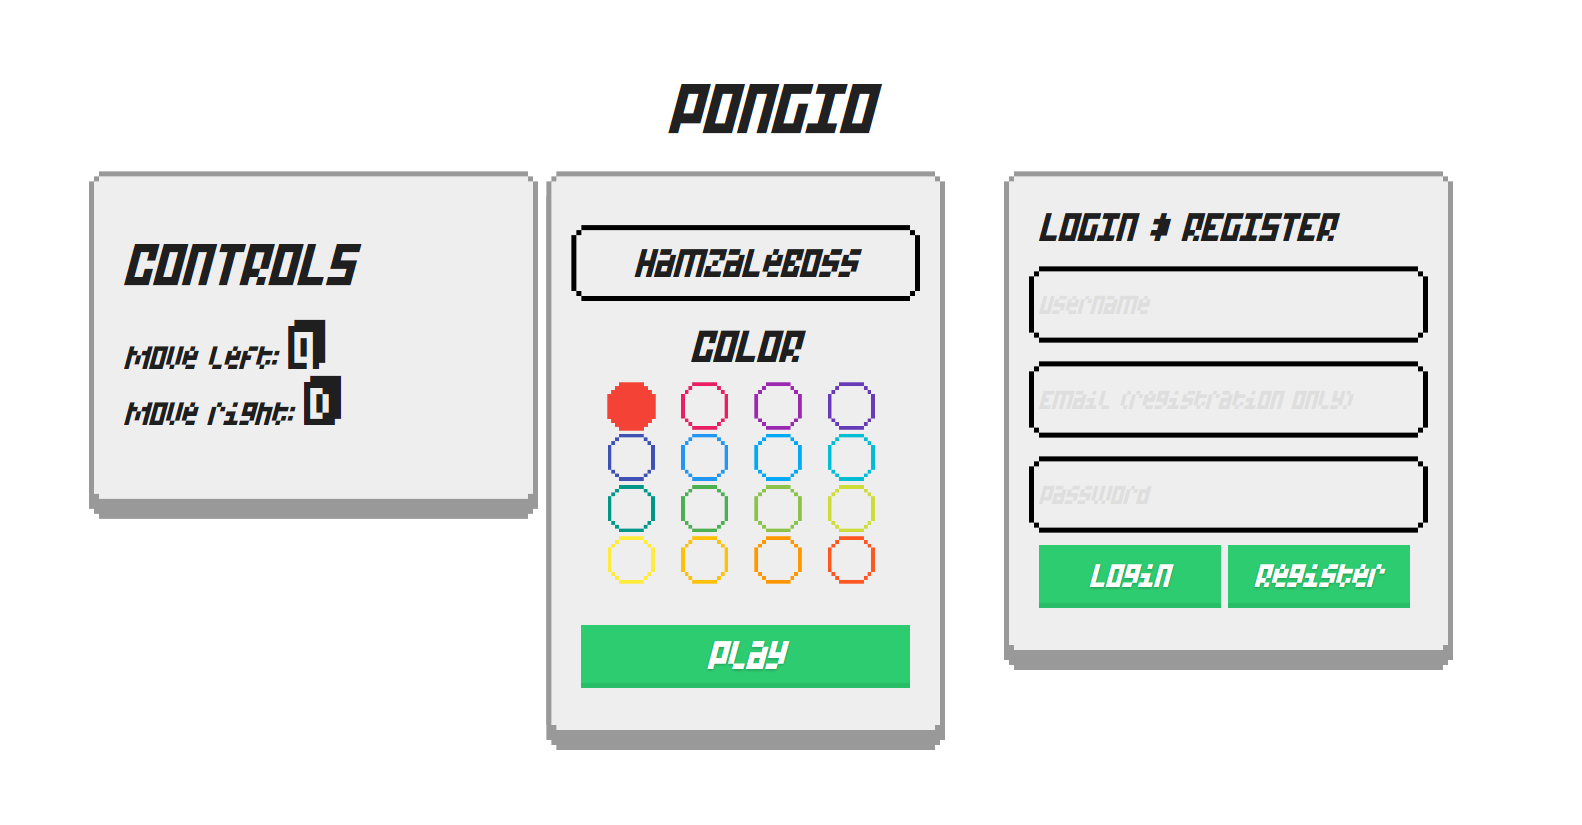
\includegraphics[width=10cm]{images/Capture3}
  \caption{Illustration de notre page de lancement aux graphismes pixélisées. Au centre, on voit le menu qui demande le pseudo et la couleur du joueur. À gauche, on indique les contrôles du jeu. À droite, un formulaire d'inscription et de connexion.}
  \label{fig:deux-image}
\end{figure}

Un de nos objectifs de départ était de permettre une interaction simple et immersive entre les joueurs durant le jeu. C'est donc dans cette optique qu'on a commencé par y intégrer un chat et un classement. On ne souhaitait pas suivre le schéma des autres jeux ".io" mais ces deux aspects nous semblaient essentiels pour l'enrichissement de l'expérience de jeu et des interactions entre joueurs.


Dans la continuité de notre démarche de changement, nous avons complètement changé le style de la fenêtre de conversation et du classement pour les accorder a notre charte graphique. Ce n'était guère notre choix de départ, nous comptions nous orientés vers un design moderne avec fond ébène mais le résultat ne s'accordé pas avec le plateau de jeu en plein milieu. Voici donc une illustration de notre classement et de notre chat pixélisés:

\begin{figure}[H]
  \centering
  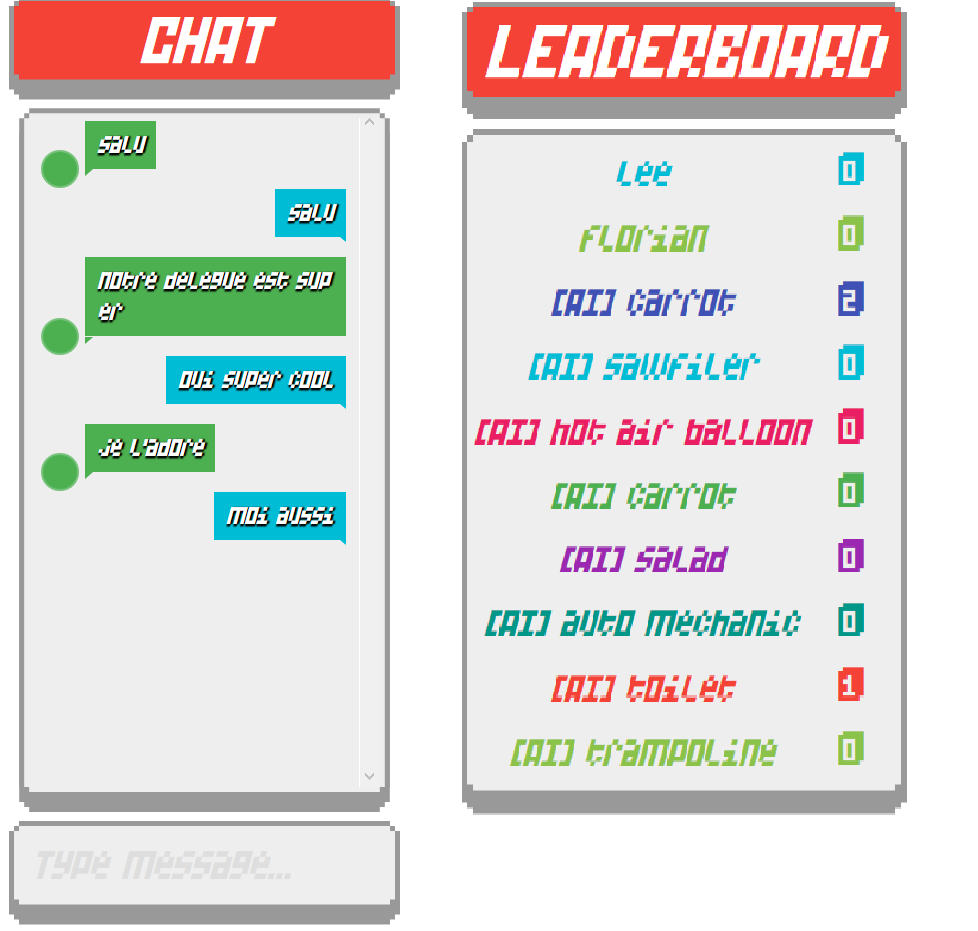
\includegraphics[width=10cm,height=7cm]{images/Capture6}
  \caption{Illustration de notre chatbox à gauche et de notre classement à droite.}
  \label{fig:trois-image}
\end{figure}

Finalement nous avons implémenté de multiples modes de jeu qui alternent après une partie de deux minutes. Pour permettre ce changement nous avons ajouté un compte à rebours juste en dessous de notre classement. Les modes de jeu se composent alors d'un mode 1vs1 simple, en d'autres termes, le mode dit "classique", un mode 2vs2 pour qui voient s'affronter deux équipes de deux joueurs, un mode avec 5 joueurs en forme d'hexagone et un mode avec 10 joueurs en forme de décagone. Voici une représentation des différents modes implémentés dans notre jeu:

\begin{figure}[!h]
  \centering
  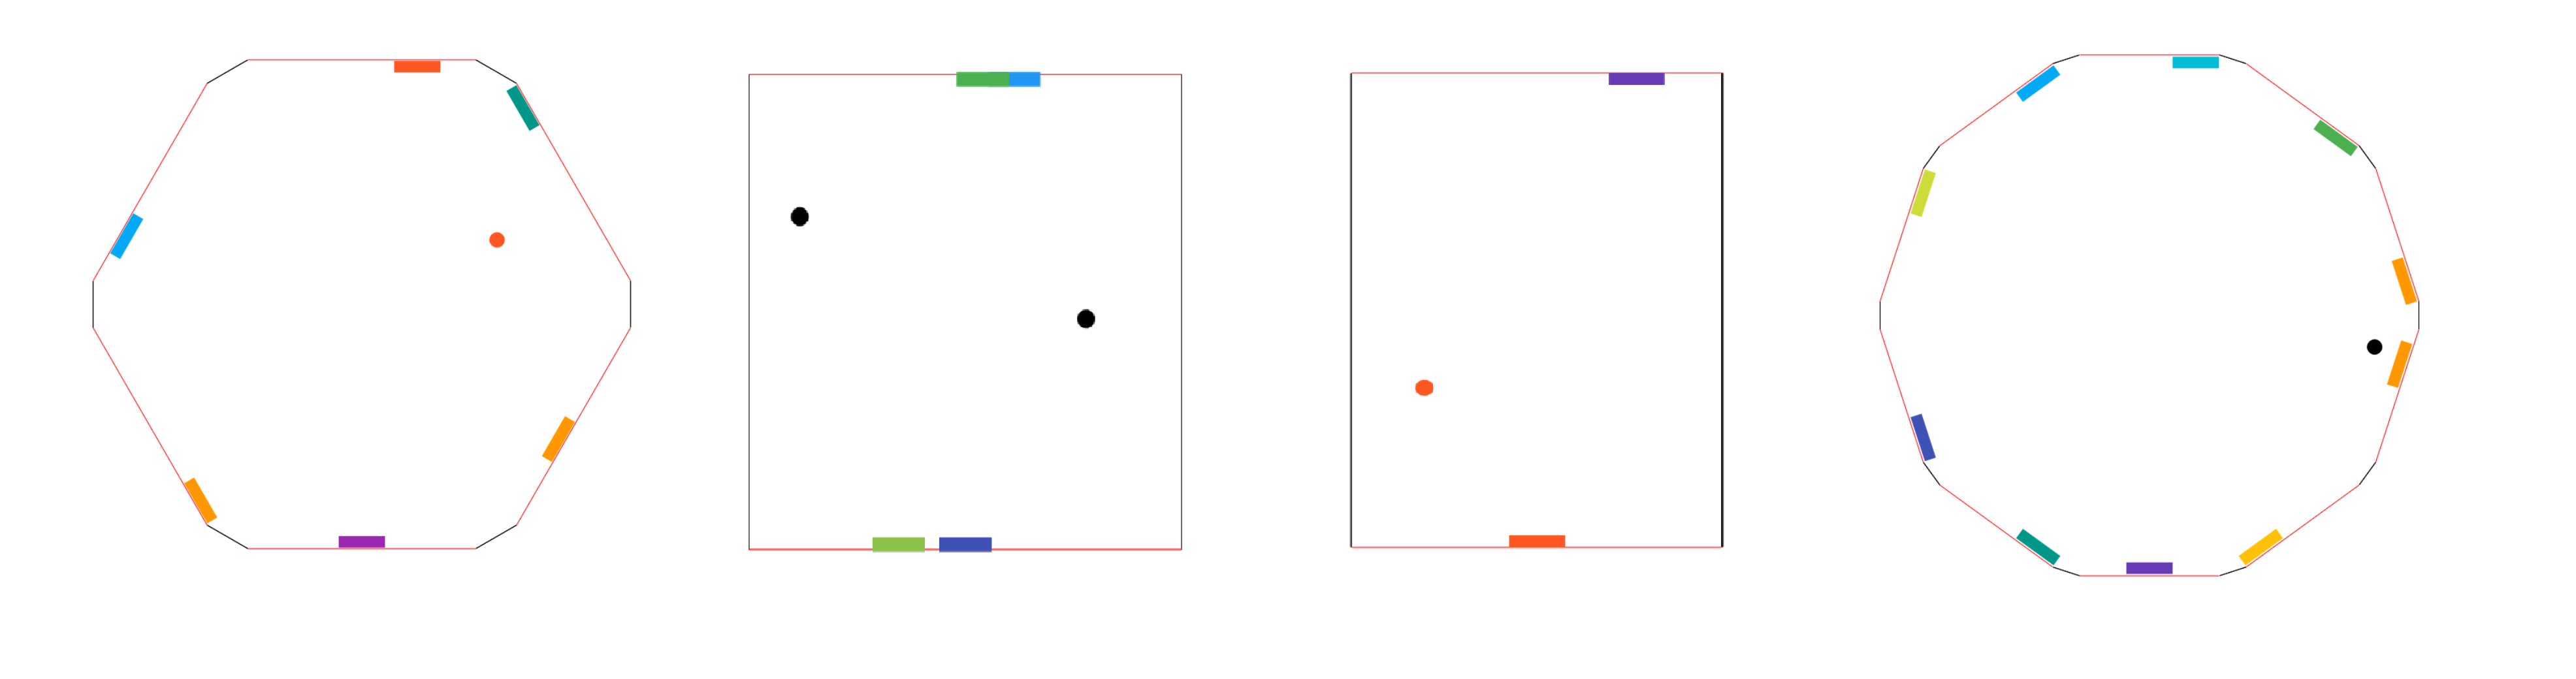
\includegraphics[width=15cm]{images/Capture11}
  \caption{Illustration des différents modes.}
  \label{fig:quatre-image}
\end{figure}


\section{Gestion du projet}

À la différence de plusieurs autres groupes de TER qui ont utilisé la méthode classique de gestion de projet, nous avons développé notre projet grâce à la méthode agile.


La méthode agile utilise le concept de développement itératif qui consiste à découper le projet en plusieurs parties que l’on appelle \emph{itérations} ou \emph{sprints}.


Ces \emph{sprints} sont en fait des sous-projets prédéfinis à l'avance avec les membres du groupe ou éventuellement avec le client en précisant les différentes parties qui seront développées en priorité. Avec le professeur référant, le groupe établit alors les tâches nécessaires pour le développement de ces parties.


Le but est de découper le projet en "itérations" plutôt que de tout prévoir et planifier tout en sachant que des imprévus arriveront en cours de route.\\
Les avantages du développement itératif sont avant tout une meilleure qualité de la communication entre les membres du groupe ou possiblement le client avec la possibilité de clarifier les exigences de chacun au fur et à mesure, une meilleure visibilité pour le groupe ou le client sur l’avancement des différentes tâches, un meilleur contrôle de la qualité car les tests du code sont effectués en continu, une meilleure détection des risques car les risques seront détectés plus tôt; une motivation et une confiance entre le groupe dû entre autres à la satisfaction d’avoir atteint un objectif fixé et enfin un contrôle des coûts plus minutieux car ainsi le projet peut être arrêté s’il n’y a plus de budget.


Notre projet a tout de suite démarré par la création d'un compte GitHub pour mieux gérer le partage du travail dans tout le groupe et pour permettre une meilleure coordination entre chacun de nous. GitHub est un site d'hébergement et de gestion de code source. De plus nous avons chacun travaillés sur des branches différentes pour éviter de saturer et de fausser notre code principal.